\chapter{Social engineering i praktiken}

Detta kapitel behandlar social engineering ur ett praktiskt perspektiv. Inledningsvis diskuteras hur social engineering påverkar organisationer och infrastrukturer med hög säkerhetsnivå. Därefter presenteras relevanta fallstudier av social engineering-relaterade incidenter, där angreppsmetoder och konsekvenser analyseras i sitt sammanhang. Avslutningsvis behandlas de bredare konsekvenser som social engineering-attacker kan ha som följd för organisationer och samhällen.

\section{Social engineering i samhällskritiska system}
Social engineering utgör ett särskilt allvarligt hot när den riktas mot samhällskritiska system och infrastrukturer. Sådana system omfattar exempelvis energiförsörjning, finansiella tjänster, hälso- och sjukvård, telekommunikation och offentliga förvaltningar. Dessa samhällskritiska system kännetecknas av sin höga komplexitet, omfattande digitala sammankoppling och beroende av både tekniska och mänskliga processer \cite{cybersakerhet_kommuner, washo2021interdisciplinary, enisa2018cybersecurity_culture}. 

För dessa system är tillgänglighet, integritet och konfidentialitet centrala säkerhetsprinciper. Social engineering påverkar dessa principer genom att manipulera den mänskliga komponenten istället för att direkt fokusera på infrastrukturens teknik. Enligt \cite{se_threat_defense_survey, algarni2019se_survey} fungerar social engineering som en initial intrångsvektor, där användningen av olika angreppsmetoder möjliggör tekniska intrång i system och nätverk. För dessa system innebär detta exempelvis att en anställd avsiktligt eller oavsiktligt lämnar ut autentiseringsuppgifter, godkänner en obehörig åtkomstbegäran eller genomför en lösenordsåterställning. 

\begin{figure}[H]
    \centering
    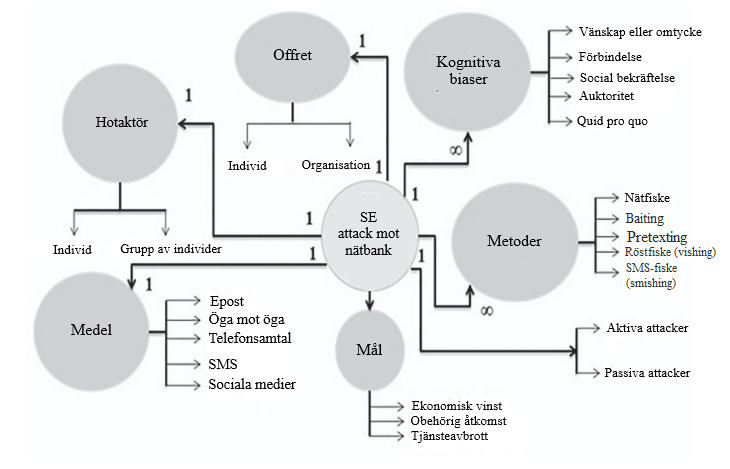
\includegraphics[width=\textwidth]{Bilder/SE33}
    \caption{En översättning av bilden \textit{Ontology model of social engineering in e-banking} \cite{gururaj2024social_engineering}.}
    \label{fig:se_samhällskritiska}
\end{figure}

För att motverka social engineering inom samhällskritiska system använder många organisationer avancerade tekniska skyddsåtgärder, såsom flerfaktorautentisering (MFA), nätverkssegmentering och intrångsdetektionssystem. Oavsett dessa avancerade system fortsätter den mänskliga faktorn inom systemen att utgöra en betydande sårbarhet \cite{washo2021interdisciplinary, albladi2018defense_mechanisms}. Särskilt utsatta är operativa gränssnitt där mänskligt beslutsfattande kombineras med tekniska processer, såsom helpdesk-funktioner, administrativ åtkomsthantering och leverantörskommunikation. Som tidigare betonats av \cite{washo2021interdisciplinary, enisa2018cybersecurity_culture} påverkar organisatoriska strukturer och arbetsprocesser hur motståndskraftiga dessa gränssnitt är mot manipulation. 

\section{Fallstudier av social engineering-relaterade incidenter}
För att förtydliga hur social engineering framträder i praktiken analyseras i detta avsnitt utvalda verkliga incidenter. Fallstudierna syftar till att illustrera hur social engineering kan användas för både ekonomisk vinning och strategisk samhällspåverkan. Angreppsmetoder som tidigare presenterats kommer också att behandlas, där attackerna tillämpas i organisatoriska och politiska sammanhang. Fallstudierna kommer också att illustrera hur avancerade tekniska verktyg, som AI, kan förstärka manipulationens effektivitet.

\subsection{Arup djupfejk-bedrägeri}
Under 2024 utsattes det internationella teknikkonsultföretaget Arup för en omfattande social engineering-attack där AI användes för att genomföra ett avancerat djupfejk-bedrägeri \cite{guardian_arup_2024, bbc_arup_2024}. Händelsen lyfte fram hur AI i moderna social engineering-attacker kan förstärka traditionella manipulationsmetoder och skapa nya säkerhetsutmaningar för organisationer.

En anställd vid företagets kontor i Hongkong mottog ett meddelande som påstods komma från företagets ekonomichef (CFO). Kort därefter deltog den anställde i ett videomöte där flera personer som såg ut och lät som företagets chefer deltog. Enligt rapportering från både BBC och The Guardian var samtliga deltagare i videomötet AI-genererade djupfejkar, där hotaktörerna hade manipulerat både bild och ljud för att imitera verkliga personer inom organisationen \cite{guardian_arup_2024, bbc_arup_2024}. Under mötet anvisades den anställde att genomföra ett antal banköverföringar till olika konton. Totalt överfördes cirka 20-25 miljoner amerikanska dollar genom flera separata transaktioner innan bedrägeriet upptäcktes \cite{guardian_arup_2024, bbc_arup_2024}. Arup bekräftade senare incidenten och att den utgjorde en form av teknologiskt förstärkt bedrägeri.

Ur ett cybersäkerhetsperspektiv visar Arup-fallet hur social engineering kan utvecklas genom integration av AI. Attacken byggde inte endast på utnyttjandet av tekniska sårbarheter i nätverk eller system, utan också på manipulation av en anställds förtroende i en situation som framstod som legitim \cite{algarni2019se_survey}. Denna specifika incident överensstämmer med tidigare forskning från \cite{algarni2019se_survey} där social engineering påstås fungera som en intrångsvektor, där hotaktören utnyttjar mänskligt beslutsfattande istället för tekniska brister.  

Vidare hänvisar incidenten till utvecklingen av AI-stödd social engineering, där generativa modeller används för att producera språkligt och visuellt övertygande innehåll \cite{zhang2024digital_deception}. Genom att kombinera djupfejkteknik med organisatorisk kontext skapade hotaktörerna ett trovärdigt scenario där traditionella tekniska säkerhetsåtgärder inte räckte till. Fallet bekräftar även \cite{algarni2024comprehensive_taxonomy} där det observeras att moderna social engineering-attacker ofta kombinerar tekniska och sociala komponenter i en integrerad angreppsstrategi. Djupfejk-elementet utgjorde den tekniska komponenten, medan manipulationen av organisatoriska rutiner och beslutsprocesser utgjorde den sociala. Kombinationen möjliggjorde ett intrång utan att hotaktörerna behövde bryta igenom tekniska skyddssystem.  

\subsection{USA:s presidentval 2016}
Förutom ekonomiskt motiverade attacker har social engineering också använts för politiska ändamål. Enligt \cite{fiia2016election_hacking} har flera demokratiska val blivit utsatta för koordinerade cyber- och desinformationsoperationer där teknik och psykologisk manipulation har kombinerats för att kontrollera informationsflödet. En av de mest dokumenterade exemplen på hur social engineering kan användas inom demokratiska val är USA:s presidentval 2016.

Under valrörelsen genomfördes riktade spjutfiske-attacker mot politiska kampanjorganisationer, som exempelvis Democratic National Committee (DNC). Genom nätfiskeattacker som utgav sig för att vara legitima säkerhetsvarningar lyckades hotaktörerna få tillgång till interna e-postkonton. Efter det lyckade intrånget började den stulna kommunikationen att publiceras via externa plattformar. Enligt \cite{fiia2016election_hacking} användes den stulna informationen strategiskt för att skapa uppmärksamhet på sociala medier och orsaka politisk polarisering och misstro. Syftet med attacken var därmed inte att manipulera rösträkningen rent tekniskt, utan att påverka det informationsmässiga och psykologiska klimatet kring valet. Enligt internationella utredningar kopplades attackerna i ett senare skede till statligt associerade ryska aktörer, vilket placerade incidenten i ett bredare geopolitiskt sammanhang \cite{fiia2016election_hacking}.

Fallstudiet kan ses ur ett cybersäkerhetsperspektiv som en kombination av spjutfiske och desinformationsmanipulation. Angreppets initiala fas riktade sig mot enskilda individer genom social engineering, medan senare faser syftade till en samhällelig påverkan. Här blir kopplingen till en bredare definition av social engineering tydlig. Som tidigare nämnts beskriver \cite{podgorecki1998social} social engineering som ett försök att medvetet forma sociala strukturer och kollektiva beteenden genom strategisk påverkan. I fallet med USA:s presidentval 2016 riktades attacken inte mot enskilda individer, utan mot röstare och det demokratiska förtroendet som helhet. Här betonas samma princip av \cite{fiia2016election_hacking} att, även om den tekniska valinfrastrukturen inte nödvändigtvis manipulerades direkt, kunde desinformationsoperationerna påverka hur valet uppfattades.



\section{Konsekvenser av social engineering-attacker}
Som diskuterats ovan kan social engineering medföra konsekvenser som sträcker sig långt bortom från det initiala intrånget. Beroende på kontext kan effekterna vara ekonomiska, organisatoriska, politiska eller samhälleliga. Oberoende av motivationen bakom attacken har dessa alla gemensamt att de uppstår genom manipulation av mänskligt beslutsfattande snarare än direkt tekniskt utnyttjande. 

Ur ett ekonomiskt perspektiv kan social engineering leda till allvarliga finansiella förluster. Arup-incidenten visar hur manipulation av en enskild anställd möjliggjorde överföring av miljontals amerikanska dollar utan att tekniska säkerhetssystem bröts \cite{bbc_arup_2024, guardian_arup_2024}. Liknande incidenter för med sig inte endast direkta ekonomiska förluster, utan även sekundära konsekvenser, såsom rättsliga utredningar, sanktioner och ökade säkerhetsinvesteringar. I organisatoriska sammanhang kan social engineering påverka förtroendet inom och mellan organisationer. När autentiseringsprocesser manipuleras, eller kommunikationskanaler utnyttjas, kan detta skapa osäkerhet kring rutiner och misstro mellan anställda. Enligt ENISA är säkerhetskultur och tydliga processer avgörande för att minska denna typ av organisatorisk sårbarhet \cite{enisa2018cybersecurity_culture}. Efter en incident kan organisationer tvingas att omvärdera sina säkerhetsstrategier och införa striktare kontroller, vilket kan leda till försämrad effektivitet och arbetsflöde. 

På en samhällelig nivå kan konsekvenserna vara mer omfattande. USA:s presidentval 2016 illustrerar hur social engineering kan användas för att påverka informationsmiljöer och skapa skepticism \cite{fiia2016election_hacking}. Användningen av nätfiske och informationsmanipulering bidrog till ökad polarisering och misstro kring valet. Som incidenten klart visar, var målet med attacken inte att nå ekonomisk vinst, utan att påverka kollektiv perception och politiskt förtroende. 

\begin{figure}[H]
    \centering
    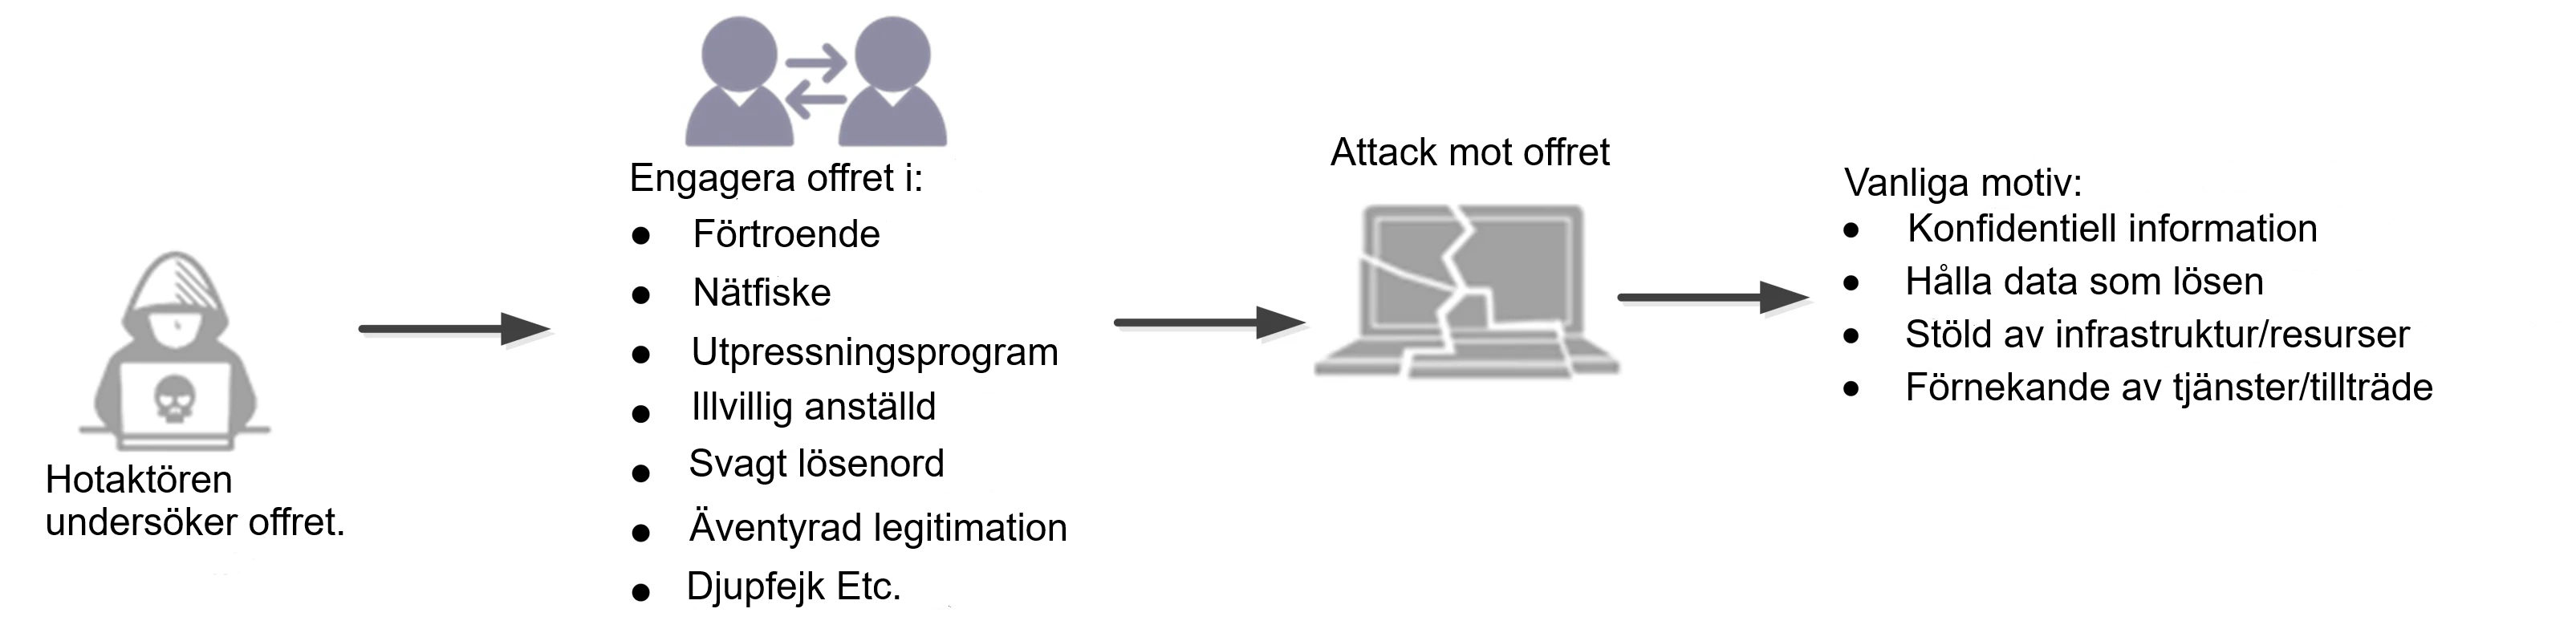
\includegraphics[width=\textwidth]{Bilder/A Study on the Psychology}
    \caption{En översättning av bilden \textit{A basic flow of social engineering-based cyberattacks} \cite{psychology_social_engineering}.}
    \label{fig:se_Konsekvenser}
\end{figure}

Från ett psykologiskt perspektiv påverkar social engineering-attacker också individers säkerhetsbeteende. Enligt \cite{psychology_social_engineering} kan manipulationen genom brådska, auktoritet och stress leda till att individer underskattar risker eller agerar impulsivt. Efter en social engineering-incident kan individers säkerhetsbeteenden förändras på olika sätt. I vanliga fall leder händelsen till ökad vaksamhet, där användare blir mer försiktiga och uppmärksamma. I andra fall kan däremot upprepade varningar, säkerhetsförfrågningar och autentiseringsmeddelanden skapa så kallad säkerhetsutmattning \cite{albladi2019training_awareness}. Fenomenet innebär att individer, på grund av stress eller vana, börjar ignorera varningar eller godkänna förfrågningar utan noggrann observation. 

Slutligen bidrar upprepade social engineering-incidenter även till en förskjutning i hotlandskapet. Enligt \cite{aldawood2019taxonomy, algarni2019se_survey, algarni2024comprehensive_taxonomy} utvecklas angreppsmetoder kontinuerligt genom tekniska verktyg och social manipulation. Detta innebär att konsekvenserna är reaktiva och att organisationer och samhällen måste konstant anpassa sig för att hantera cyberhotet.